\documentclass[
		11pt,
		a4paper,
		toc=listof, %% Abbildungs- und Tabellenverzeichnis mit ins Inhaltsverzeichnis
		bibliography=totoc %% Quellenverzeichnis mit ins Inhaltsverzeichnis
		]{scrreprt}	 %% KOMA Script

% HTWG
\usepackage{graphicx}
\usepackage{a4}
\usepackage[ngerman]{babel}
\usepackage[babel,german=quotes]{csquotes}

% Eigene
\usepackage[utf8]{inputenc} %% Umlaute
\usepackage[dua]{acronym} %% Abkuerzungsverzeichnis (nur verwendete)
\usepackage{todonotes} %% TODOs moeglich mit \todo{}
\usepackage{booktabs} %% Tabellen
\usepackage{amsmath} %% Formeln
\usepackage{listings} %% Codebeispiele
\usepackage{subfigure} %% Mehrere Bilder nebeneinander
\usepackage{hyperref} %% referenzen innerhalb und außerhalb des Dokumentes
\usepackage[headsepline]{scrlayer-scrpage} %%Numerrierung der Seiten + Kapitelnamen in Kopfzeile inkl. Trennstrich
\pagestyle{scrheadings} %% die folgenden Zeilen sorgen für die korrekte Nummerierung und deren Anzeige 
\clearpairofpagestyles %% und für die Kopfzeile mit aktuellem Kapitel etc.
\ihead{\headmark}
\cfoot[\pagemark]{\pagemark}
\automark{chapter}
\usepackage{float} %% Floatpackage um Grafik-Positionen zu forcieren
\newcommand*{\quelle}[1]{\par\raggedleft\footnotesize Quelle:~#1}
  \usepackage[
backend=biber,
style=numeric,
]{biblatex}
\addbibresource{neueBib.bib}

% Eigenes Design 
%TODO loeschen wenn default HTWG Design (was es nicht wirklich gibt) gewuuenscht ist
\usepackage[a4paper, left=2cm, right=5cm, top=2cm]{geometry}
\usepackage{setspace}
\onehalfspacing
\usepackage{mathptmx}
\usepackage[T1]{fontenc}


% KOMA script anpassungen 
%TODO entfernen wenn kein KOMA Script gewuenscht
\usepackage{scrhack}

%%%%%%%% Codebeispiele
\usepackage{color}
\usepackage{xcolor}
\usepackage{listings}
\usepackage{caption}

\setcounter{tocdepth}{2}  %% Uebreschriften bis subsectionw ins Inhaltsverzeichnis
\setcounter{secnumdepth}{3}  %% Nummerierung bis subsection


%%% Codebeispiele - Style
\DeclareCaptionFont{white}{\color{white}}
\DeclareCaptionFormat{listing}{\colorbox{gray}{\parbox{\textwidth}{#1#2#3}}}
\captionsetup[lstlisting]{format=listing,labelfont=white,textfont=white}

% Entfernt Kapitel Ueberschrift
% Bsp.
% 	ALT:
%       Kapitel 1
%       Einführung
%
% 	NEU:
% 		1 Einführung
%
\renewcommand*\chapterheadstartvskip{\vspace{-\topskip}}
\nocite{*}
\newcommand{\thema}{Wi-Seminar}
\newcommand{\forschungsfrage}{Wissenschaftliche Arbeit über das Thema LegalTech}
\newcommand{\ausgabedatum}{01.01.2018}
\newcommand{\abgabedatum}{28.02.2022}
\newcommand{\autor}{Adrian von Buttlar}
\newcommand{\matrikelnummer}{298203}
\newcommand{\erstbetreuer}{Niculin Prinz}
\newcommand{\studiengang}{Wirtschaftsinformatik}
\newcommand{\autorGeburtsdatum}{15.03.1999}
\newcommand{\autorGeburtsort}{Stuttgart}



\begin{document}
%% Nummerierung aus
\pagenumbering{gobble}

% HTWG Templates fuer Titelseite etc.

\begin{titlepage}

\vspace*{-3.5cm}

\begin{center}

\includegraphics[width=5cm]{htwg/htwg-logo}

Fakultät Informatik \\
Fachbereich Wirtschaftsinformatik
\end{center}

\vspace*{1.5cm}

\begin{center}
	\huge{
		\textbf{\thema} \\[1cm]
	}
	\normalsize{
		\textbf{\forschungsfrage} \\[2cm]
	}
\end{center}
\begin{tabular}{p{6cm}p{5cm}}
                 \bfseries{Name:} & \autor \\\\
                 \bfseries{Erstkorrektor:} & \erstbetreuer \\\\
                 \bfseries{Abgabetermin:} & \abgabedatum \\\\
\end{tabular}
\\[1cm]
\begin{flushright}
	Konstanz, \abgabedatum \\[0.5cm]
\end{flushright}
\end{titlepage}
\pagenumbering{Roman}
\tableofcontents
\addcontentsline{toc}{chapter}{Inhaltsverzeichnis}

\clearpage
%% Starte Paginierung
\linespread{1.25}
\pagenumbering{arabic}

\chapter{Einleitung}

\section{Relevanz und Ziel der Arbeit}
Seit 2017 der deutsche Anwaltstag als einer der Hauptthemen Legal Tech angeführt hat, hat das Thema für den Rechtssektor rasant an Bedeutung gewonnen. In einer Branche die laut Statista im Jahr 2018 28,82 Mrd Euro erwirtschaftet hat, spielt Technik eine immer größer werdende Rolle \footfullcite{StatistikUmsatz}. Laut des STAR Bericht der Bundesrechtsanwaltskammer 2020 sind 77\% der befragten Anwälte überzeugt, dass Legal Tech einen entscheidenden Vorteil für ihre Kanzlei bietet \footfullcite{STARStatistik}. Die Leitfrage der Arbeit lautet: Hat Legal Tech das Potential, den Markt zu verändern und falls ja, wie weit ist ein Fortbestehen der alten Methoden neben Legal Tech möglich?
\section{Methodik}

Für diese Arbeit wurde Fachliteratur über Google Scholar sowie Literatur aus der Hochschulbibliothek der Hochschule für Technik Wirtschaft und Gestaltung Konstanz verwendet. Hauptsächlich wurde mit ,, Legal Tech
und Legal Robots - Der Wandel im Rechtsmarkt
durch neue Technologien
und künstliche Intelligenz '' von Jens Wagner\footfullcite{LegalRobots} in der zweiten Auflage gearbeitet. Dieses bietet aus technischer Sicht den umfänglichsten Einblick in das Thema Legal Tech und wurde außerdem von verschiedenen Quellen zitiert und deshalb ausgewählt. Darauf aufbauend wurde die Rückwärtssuche angewandt. Hier durch, und durch Veröffentlichungen des selben Verlags wurden die meisten Quellen selektiert. Alle genutzten Quellen wurden zwischen 2018 und 2022 veröffentlicht. Dies liegt dem Fakt zu Grunde, dass Legal Tech erst seit Mitte der 2010er in Deutschland an Relevanz gewinnt. Somit wurde auch erst wenig zitierfähige Fachliteratur veröffentlicht. Die
Arbeit bietet ein Gesamtbild über das Thema Legal Tech und dient
nicht als Handlungsempfehlung. Alle getroffen Schlüsse sind lediglich persönliche Einschätzungen aufgrund des in der Literatur gewonnenen Wissens.

\section{Aufbau der Arbeit}

Zunächst wird der Begriff Legal Tech definiert und eine grobe Kategorisierung der verschiedenen Einsatzbereiche beschrieben. Das nächste Kapitel beschäftigt sich mit eben diesen Einsatzbereichen. Diese werden in wiederum verschiedene Typen eingeteilt und innerhalb dieser werden die Methoden des Typs beschrieben. Im darauf folgenden Kapitel wird auf die Auswirkung dieser Methoden eingegangen und die sich dadurch ergebende Veränderung des Marktes beschrieben. Anschließend werden die durch Legal Tech entstandenen rechtlichen Komplikationen erläutert. Abschließend wird ein Fazit und ein Ausblick in die Zukunft gegeben. 

\chapter{Grundlagen}
Den Begriff Legal Tech trifft man in der heutigen Rechtsbranche immer wieder. Dort ist Legal Tech
ein Trendthema wie künstliche Intelligenz in der IT. Alle diejenigen, die sich am Markt positionieren
wollen, beschäftigen sich mit dem Thema Legal Tech. ,,Definieren kann man Legal Tech als Abkürzung für
den Ausdruck Legal Technology, der die Verbindung von Technologie und Recht im Arbeitsalltag bezeichnet.''\footfullcite[S. 15]{LegalTech}
In diesem Begriff wird die konservative Rechtsbranche mit der progressiven IT- und Technikbranche vereint.
Es wird als das Tool der Zukunft für die Rechtsberatung gehandelt. Anwälte und Richter versprechen sich durch
Legal Tech effizientere, kostengünstigere und konstant qualitativ hochwertige Rechtsberatung und die Möglichkeit, dort rechtliche Unterstützung zu bieten, 
wo es bis jetzt nicht wirtschaftlich sinnvoll war.
Ob durch Legal Robots, Chatbots, Smart Contracts oder einfache digitale Aktenverwaltung: Ziel ist es, alle repetitiven Prozesse
zu automatisieren. Dafür bietet sich das Rechtswesen an, da dort Prozesse zu meist sich wiederholend und immer gleichbleibend sind.
Die Ansprüche sind die selben, die Abläufe sind die selben, lediglich der Mandant ist ein Anderer.

\section{Definiton Legal Tech}
Der Begriff Legal Tech wird in der Branche und in der dazu passenden Literatur verschieden eingesetzt.
Manche meinen mit dem Begriff lediglich das Digitalisieren (Digitisieren) von vorhandenen Prozessen.
Beispielsweise wird der Schriftverkehr nicht mehr per Post, sondern über das besondere elektronische Anwaltspostfach sowohl dem Gericht als auch dem
Gegner zugestellt. Andere wiederum meinen mit Legal Tech die vollautomatisierte Bearbeitung von Rechtsfällen. Um das Ganze
einordnen zu können, hat Oliver Goodenough eine Kategorisierung eingeführt, die es ermöglicht die verschiedenen Ansprüche
an Legal Tech eingliedern zu können. Goodenough kategorisiert Legal Tech in 3 Kategorien: \nameref{Legal Tech 1.0}, \nameref{Legal Tech 2.0}, \nameref{Legal Tech 3.0} \footfullcite{Kategoirien}

\subsection{Legal Tech 1.0} \label{Legal Tech 1.0}
Unter Legal Tech 1.0 (u.a. auch OfficeTech genannt) werden Technologien zusammengefasst, die den im Rechtssektor arbeitenden Menschen den Alltag erleichtern. Es ist die oberste und vermeintlich simpelste Form des Legal Techs. Dazu gehört Aktenverwaltungssoftware, Dokumentenerstellungssoftware und Software zur Unterstützung von Rechtsrecherche. Aber auch Online-Vermarktung, -Recruitment oder -Marktplätze zur Suche von Terminsvertretung (Legal Outsourcing) werden unter dem Begriff Legal Tech 1.0 geführt. Anders ausgedrückt sind es Tools, die wir bereits aus anderen Branchen kennen und für den Rechtssektor angepasst wurden. 
\subsection{Legal Tech 2.0} \label{Legal Tech 2.0}
Legal Tech 2.0 strebt die Ersetzung des menschlichen Juristen innerhalb des bestehenden Systems an. Das soll durch automatisierte Rechtsdienstleistung bewerkstelligt werden. So sollen Programme einzelne Schritte der bestehenden Prozesse übernehmen. Dokumentenauslese, automatische Erstellung juristischer Dokumente, Einordnung der Rechtsansprüche und Erfolgsaussichten, Analyse der Urteile zu einem bestimmten Fall an einem bestimmten Gericht, Vertragserstellung auf Grundlage eines Fragenkataloges an den Mandanten. All dies soll ohne Eingriff eines Juristen erfolgen.

\subsection{Legal Tech 3.0} \label{Legal Tech 3.0}
Legal Tech 3.0 soll das ganze Rechtssystem revolutionieren. Hierbei soll nicht wie in \nameref{Legal Tech 2.0} einzelne Schritte des bestehenden Systems automatisiert werden, sondern das ganze System neu formiert werden. Ziel ist es, komplexe und umfangreiche Rechtsdienstleistungen vollautomatisch abzuschließen. Beispielsweise soll eine autonome Sichtung, Bewertung und auch Verhandlung eines bestimmten Falles ermöglicht werden. Unter diese Kategorie fallen 'Legal Robots / Laywers' oder aber 'Smart Contracts' welche im späteren Verlauf der Arbeit noch genauer beschrieben werden.

\section{Verschiedene Perspektiven auf Legal Tech}
Die von Goodenough eingeführten Kategorien zeigen die Fortschrittlichkeit von Legal Tech an. Dies beschreibt aber leider nur einen Aspekt des Legal Tech's. Waltl, B., Jacob, K. \& Schindler, D haben in Ihrem Artikel ,,Legal Tech – interdisziplinär und kollaborativ'' eine weitere Betrachtungsweise veröffentlicht. Diese Unterteilen Legal Tech auf Sechs verschiedene Perspektiven. Die dazu gelieferte Abbildung soll anschaulich zeigen, aus welchen verschiedenen Aspekten Legal Tech zusammengestellt ist. Abb.\ref{img:Legal Tech – interdisziplinär und kollaborativ}

\begin{figure}
	\centering
	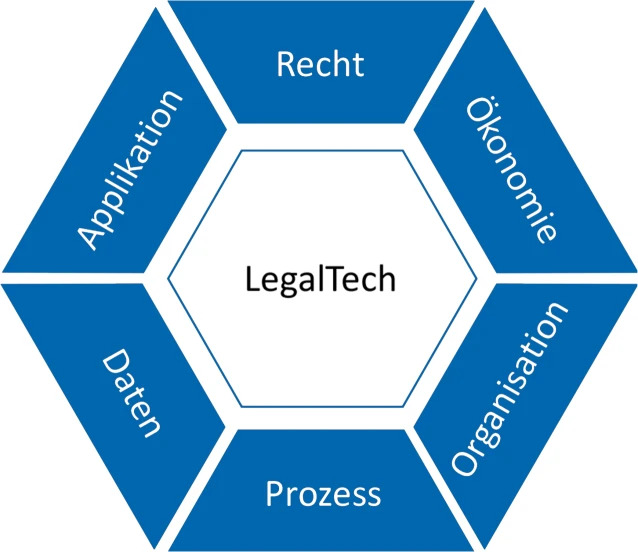
\includegraphics[height=4cm]{Bilder/35764_2020_300_Fig1_HTML.jpg}
	\caption{Zentrale Aspekte von Legal Tech }
	\cite{LegalTechKategorien}
	\label{img:Legal Tech – interdisziplinär und kollaborativ}
\end{figure}

Diese Aspekte bestehen aus 5 Punkten: \footfullcite{LegalTechKategorien}
\subsection{Rechtliche Sicht}
Aus der rechtlichen Sicht muss betrachtet werden, ob ein Einsatz der gegebenen Technologie in diesem bestimmten Gebiet gestattet ist und ob er tatsächlich einen Mehrwert zur Lösung des rechtlichen Problems leistet.

Gerade bei komplexeren oder fachübergreifenden Themen sollte besonders Vorsicht geboten sein. Anwendungen können zu meist nur für rechtliche Themen eingesetzt werden, in denen rechtliche Klarheit besteht. Da die Rechtsprechung in Deutschland nicht einheitlich geregelt ist und Gesetze auslegbar sind, kann es durchaus vorkommen, dass der selbe Rechtsfall an zwei verschiedenen Gerichten unterschiedlich entschieden werden. Hier kommt der Faktor Mensch ins Spiel. Das sollte vor dem Einsatz von Legal Tech zur Unterstützung unbedingt beachtet werden

\subsection{Ökonomische Sicht}
Kann Legal Tech die Effizenz meines Unternehmens erhöhen und gleichzeitig die Risikien minimieren? Kann dadruch ein monetäre Mehrwert entwickelt werden?

Nicht nur der Rechtssektor sondern fast jede Branche setzt auf Optimierung der Prozesse durch technische Unterstützung. Durch den immer steigenden wirtschaftlichen Druck kann ein solcher Vorteil durchaus entscheidend sein. Eine fortschrittliche technische Unterstützung kann das Unternehmen auch für potentielle zukünftige Mitarbeiter attraktiv machen und damit auch einen ökonomischen Vorteil bieten. 

\subsection{Organisationssicht}
Einführung solcher Technologie kann auch eine Veränderung der Organisationsstruktur mit sich führen. Ein Vergleich mit der Einführung eines Enterprise Resource Planning-Systems in Handelsfirmen ist durchaus möglich. Viele Prozesse sollten sich demnach an das System angleichen, um den maximalen Nutzen zu entwickeln. Hierbei ist ein gutes Change Management notwendig \footfullcite{LegalTech}. Dabei sollte darauf geachtet werde, dass die Personen, deren Aufgaben durch die neue Technologie erledigt werden, eine andere passende Aufgabe erhalten. Das erhöht die Akzeptanz der Technik unter den Mitarbeitern


\subsection{Prozesssicht}
Welche Prozesse sollen von Legal Tech unterstützt werden?

Um diese Frage zu beantworten, müssen zunächst die Abläufe und Prozesse genaustens festgelegt und modelliert werden. Erst dann ist eine zuverlässige Beantwortung dieser Frage möglich. 

\subsection{Applikationssicht}
Welche Aufgaben sollen von der Technologie erledigt werden und können diese von bestehenden Anwendungen erfüllt werden oder müssen neue Anwendungen entwickelt zur Verfügung gestellt werden.

\subsection{Datensicht}
Datensicht: Liegen notwendige Daten vor oder können und dürfen diese erhoben, verarbeitet und gespeichert werden, damit die Technologie ihr volles Potenzial entfalten kann?

Alle Applikationen im Legal Tech brauchen in einer Weise Daten. Ohne Daten kann kein mehr wert geschaffen werden. Diese Daten müssen dann auch zwischen verschiedenen Anwendungen verteilt werden können. Daher ist es wichtig, dass im Legal Tech-Sektor nicht nur auf die Datenmasse und Integretät geachtet wird, sondern selbstverständlich auch auf die rechtlichen Grundlagen dafür.

\chapter{Einsatzbereiche von Legal Tech} \label{Einsatzbereiche von Legal Tech}
Im folgenden Abschnitt wird Bezug auf die einzelnen Bereiche des Legal Tech genommen. Ferner wird beschrieben wie und wo Legal Tech Personen im traditionellen Rechtssektor unterstützt. Jeder Unterpunkt beschreibt eine bestimmte Art des Legal Tech's.

\section{Dokumente}
In den folgenden Unterpunkten sind Legal Tech-Einsatzbereiche zusammengefasst, die den Juristen bei der Bewältigung ihres Alltags helfen. Allgemein kann man diese unter \nameref{Legal Tech 1.0} zusammenfassen.
\subsection{Dokumentenerstellung}
Die offensichtlichste und einfachste Weise, wie Technologie einen Anwalt oder einen Richter unterstützen kann, ist in der Dokumentenerstellung. Es liegt in der Natur der Sache, dass im Rechtswesen viele und vor allem lange Schriftstücke erstellt und verschickt werden. Hierfür benötigt es Software, die es den Juristen ermöglicht schnell und fehlerfrei Schriftstücke zu erstellen. Oft reichen in größeren Kanzleien nicht nur einfache Word-Vorlagen. Da Schriftsätze oft über mehr als 100 Seiten verfügen und penible Genauigkeit erfordern, wird hier vom Markt speziell für den Rechtssektor ausgelegte Software bereit gestellt. Diese verfügt dann normalerweise zum einen über Funktionen zum erstellen solcher Dokumente, zum anderen auch über Funktionen zum kreieren von Musterstücken, die dann zur Massenproduktion eingesetzt werden können. Hierfür wird meistens eine Kombination aus Microsoft Word und dem in der Kanzlei vorhandenen Aktenverwaltungssoftware genutzt.

 \subsection{Dokumentenanalyse}
Zum Beruf eines Juristen gehört es nicht nur selber Schriftstücke zu erstellen, sondern auch auf solche der Gegenseite zu antworten. Da wie bereits erwähnt diese Schriftstücke üblicherweise sehr lang sind, würde es auf dem traditionellen Weg sehr lange dauern, alle diese Schriftstücke vollumfänglich zu lesen. Hierfür bietet der Legal Tech-Markt auch Lösungen: Programme, die dazu geschaffen wurden, zunächst den Adressat / Fall des juristische Werks herauszufinden und dann zu analysieren und deren Kernaussage heraus zu filtern. Hierbei wird zum Beispiel auf fehlende Kriterien, fehlerhafte Klauseln oder generelle Risiken geprüft. Das bekannteste Programm zur Dokumentenanalyse ist Juristische Textanalyse der DATEV eG.

\subsection{Datenbanken und Wissensmanagement-Systeme}
Zur Klärung des Sachverhaltes und Herausfiltern etwaige Ansprüche benötigt es juristischer Kenntnisse. Da diese aber sehr umfangreich und niemals vollumfänglich präsent seien können, bedarf es auch hier an Unterstützung. Früher war hierfür eine umfangreiche Bibliothek mit abermals vielen Aufzeichnungen nötig. Lange Recherchen nach den richtigen Schriftstücken gehörten zum juristischen Beruf dazu. Dafür bietet der Legal Tech-Sektor Abhilfe. Datenbanken und Wissensmanagment-Systeme, die den Juristen in seiner Arbeit unterstützen sollen, werden hierfür angeboten. Es werden jegliche Urteile, Gesetze, Kommentare und Aufsätze zu einem bestimmten Thema gesammelt und dem Juristen auf Knopfdruck angeboten. Dadurch lässt sich dieser Teil der Arbeit äußerst effizient gestalten. Vor allem im anglo-amerikanischen Rechtskreis sind diese Datenbanken essenziell. Dort ist das Rechtssystem auf Fallrecht aufgebaut, das heißt die primäre Rechtsquelle ist nicht wie in Deutschland die generellen Gesetzte, sondern die richterlichen Entscheidungen konkreter Fälle. Deshalb müssen dort für Rechtsstreite so genannte Präzedenzfälle gesucht werden, die auf den eigenen Rechtsstreit anwendbar sind. Im europäischen Raum gilt kodifiziertes Recht, dass heißt es wird nach dem Gesetz und nicht nach vorher verhandelten Fällen entschieden. Somit müssen für diese Anwendungsfälle verschiedene Datenbanken angeboten werden. Die bekannteste Deutsche Rechtsdatenbank gehört dem Beck Verlag und heißt beck-online.

\section{Vermittlung}
Vermittlung und Findung des richtigen Partners ist immer der erste wichtige Schritt zur Lösung eines Problems.
In diesem Abschnitt werden Techniken genannt, die alle am Rechtssektor teilnehmenden Personen bei der Findung des richtigen Partners unterstützen sollen.
\subsection{Plattformen für Anwaltsleistungen} \label{Plattformen}
Durch das Internet werden viele Dienstleistungen, die früher lokal (,,vom nächst Besten'') erledigt wurden, nicht mehr unbedacht vergeben. Selbes gilt auch für den Rechtssektor. Auch hier wird mittlerweile vom Mandanten bewertet, verglichen und abgewogen. ,,Durch Abschaffung der Singularzulassung der Rechtsanwäte [...] [Gibt es] die Möglichkeit, anwaltliche Dienste ohne örtliche Beschränkungen anbieten zu können [...]''. \footfullcite[S. 11]{LegalRobots} Im Folgenden werden verschiedene Plattformen beschrieben, durch die sich der anwaltliche Beruf verändert hat.
\subsection{Anwaltsportale und Anwaltssuchmaschinen} \label{Anwaltsportale}
Anwaltsportale und Anwaltssuchmaschinen sind, wie es der Name schon sagt, Plattformen um den passenden Anwalt zu finden. Der Anwalt selber kann ein Profil anlegen, angeben welche Rechtsgebiete er abdeckt und eigene Veröffentlichungen zu bestimmten Themen bekannt geben. User, die auf der Suche nach einem Anwalt sind, können eben solche finden und üblicherweise Bewertungen über jene abgeben. Diese Bewertungen wiederrum beeinflussen dann das Standing und Ranking des Anwalts. Der bekannteste Vertreter dieser Portale ist Anwalt.de.

\subsection{Marktplätze}
Mandanten, die Portale wie in dem Kapitel ,,\nameref{Anwaltsportale}'' beschrieben nutzen, haben oft ein ausgereiftes oder kompliziertes Rechtsproblem und suchen intensive Betreuung und Beratung. Das trifft aber nicht auf jedes Rechtsproblem zu. Oft möchten Privatpersonen nur eine rechtliche Einschätzung zu bestimmten Sachverhalten und nicht direkt ein Mandantenverhältnis zu einem Anwalt. Hierfür bieten verschiedene Plattformen eine Art Marktplatz für Rechtsberatung. Der Fragende stellt eine Art Angebot ein. Er beschreibt, was sein rechtliches Problem ist und in welchem Punkt er Hilfe benötigt. Optional kann er auch direkt einen Betrag seinem Angebot mitgeben, den er bereit wäre zu zahlen. Dann können von der Plattform bestätigte Anwälte sich diesem Problem annehmen und entweder den angebotenen Geldbetrag akzeptieren oder ein (Gegen)Vorschlag für die vom Anwalt erstellte Lösung des Problems anbieten. Bekannte Vertreter dieser Art von Marktplatz sind frage-einen-anwalt.de oder advocado.

\subsection{Terminvertretung} \label{Terminvertetung}
In der deutschen Zivilprozessordnung (ZPO) ist geregelt, welches Gericht für welche Verhandlungen zuständig ist. In §12 Allgemeiner Gerichtsstand der ZPO ist folgendes geregelt : ,,Das Gericht, bei dem eine Person ihren allgemeinen Gerichtsstand hat, ist für alle gegen sie zu erhebenden Klagen zuständig, sofern nicht für eine Klage ein ausschließlicher Gerichtsstand begründet ist.''. Dabei wird der allgemeine Gerichtsstand des Wohnsitzes (§13 ZPO)wie folgt definiert : ,,Der allgemeine Gerichtsstand einer Person wird durch den Wohnsitz bestimmt.''. Daraus folgt, dass ein Kläger für Verhandlungen immer zum Gericht des Beklagten kommen muss. Durch die Abschaffung der in \nameref{Plattformen} beschriebene Singularzulassung, kann es aber durchaus vorkommen, dass ein Anwalt aus Konstanz einen Mandanten in Kiel vertritt. Unter Berücksichtigung, dass Anwälte üblicherweise einen im Verhältnis zur restlichen Bevölkerung hohen Stundensatz haben, wäre es in diesem Fall wirtschaftlich gesehen nicht sinnvoll, dass der Anwalt selber vor Gericht erscheint. Hierfür können Anwälte andere Anwälte als Terminvertretung beauftragen. Vor der Zeit von Legal Tech war hierfür ein ausgereiftes Netzwerk notwendig, da weder Erfahrungen noch Kontakte zuverlässig öffentlich geteilt werden konnten. Diese Lücke hat Legal Tech aber durch so genannte Terminvertretungsportale geschlossen. Anwälte können hier entweder ihre Dienste für eine Anzahl von Gerichten anbieten oder aber sich für ihre Fälle passende Terminvertretungen suchen. Beispiel für ein solches Portal ist terminsvertreter.com.

\section{Automatisierte Bearbeitung}
Für alle Branchen ist es wichtig, die Effizienz zu steigern. Dies ist am einfachsten zu bewältigen, indem wiederholende Aufgaben minimiert oder standardisiert werden. Dies gilt auch für den Rechtssektor.
Unter ,,Automatisierte Bearbeitung'' werden alle Legal Tech-Bereiche zusammengefasst, die (teilweise) den Juristen oder Anwalt ersetzen sollen.

\subsection{Smart Contracts}
\label{SmartContracts}
Unter Smart Contracts werden digitale oder digitalisierte Verträge verstanden, die sich selber vollziehen. Die Vertragsbedingungen werden dabei direkt in einer Programmiersprache geschrieben. Es ist also kein Vollstrecker im herkömmlichen Sinne mehr nötig. Die zu vollstreckenden Vertragsklauseln werden abstrakt gesprochen von einer Technologie, oder zumindest nicht von einem Menschen vollzogen. Aufgrund dieser Automatisierung ist keine weitere Instanz nötig. Beispielsweise könnte ein Testament durch einen Smart Contract realisiert werden. Dann wären innerhalb Deutschlands, sofern die rechtliche Grundlage geschaffen ist, keine Testamentsvollstrecker mehr nötig. Der Smart Contract würde vollautomatisiert vollstreckt werden, sobald die Behörde den Tod eines bestimmten Menschen feststellt. Dadurch lassen sich typische Fehlerquellen ausschließen.
\subsubsection{Blockchain}
\nameref{SmartContracts} setzen eine gewisse Unveränderlichkeit voraus. Bei einem normalen Vertrag können alle Bedingungen mit Abstimmung des Vertragspartners geändert werden. Ob diese Bedingungen vollzogen wurden, können nur die beiden Parteien oder im Zweifelsfall ein Gericht entscheiden. Bei einem Smart Contract ist das ein Problem. Um dem entgegen zu wirken sollen Smart Contracts in eine Blockchain eingebracht werden. Eine Blockchain ist ein neuartiger Datenbanktyp, dessen Hauptmerkmal Dezentralisierung ist. Dadurch werden die Verträge durch Manipulation der beiden Parteien oder Dritter geschützt. Ein Beispiel für die Kombination von Smart Contract und Blockchain könnte mit der Cryptowährung Ethereum (die bereits auf der Blockchain-Technologe gebaut ist) realisiert werden. So könnte man beispielsweise einen Vertrag aufsetzen, der eine Dienstleistung enthält, die mit einem bestimmten Betrag an Etherium an eine bestimmte Adresse bezahlt wird. Sobald dann eine dritte Schnittstelle die Erbringung der Dienstleistung bestätigt, wird automatisch der vorher definierte Betrag an Etherium an die Adresse überwiesen. 
\subsection{Rechts-Generatoren}
\label{Rechts-Generatoren}
Rechts-Generatoren sind einer der ersten Schritte des \nameref{Legal Tech 2.0}. Hierbei soll der potentielle Mandant vorab einen Fragenkatalog zum Sachverhalt beantworten. Die Antworten des Mandanten werden dann durch eine Software geprüft und es findet eine automatische rechtliche Beurteilung statt. Sollte ein Rechtsanspruch vorliegen, so erstellt die Software üblicherweise auch automatisch ein passendes Schriftstück, das dann nur noch von einem Anwalt verschickt werden muss. Beispiele hierfür sind Start-Ups wie MyFlyRight oder RefundRebel. Diese nutzen solche Rechts-Generatoren, um einen Markt zu bedienen, der auf herkömmlicher Weise nicht wirtschaftlich bedient werden könnte. Die Streitwerte wären zu gering, dass ein Anwalt sich damit auseinander setzen könnte und die anwaltlichen Kosten den durch die Klage erstreitbaren Mehrwert übersteigen würden. \footfullcite[S. 27]{LegalRobots}. Beispielsweise nutzt RefundRebel solche Rechts-Generatoren, um automatisch das Erstattungsformular der Deutschen Bahn AG auszufüllen.

\subsection{Chatbots}
Einen Chatbot kann man beschreiben, als ein softwareunterstütztes Dialogsystem, das nach bestimmten Regeln oder mit Hilfe künstlicher Intelligenz mit Menschen interagiert, sei es durch Texteingabe, Sprache oder Gestik. Der Vorteil von Chatbots ist, dass man dem potentiellen Mandanten eine 24/7 Versorgen vortäuschen kann. Chatbots ermöglichen es, jederzeit auf Anfragen zu reagieren, diese einzuordnen und in vielversprechenden Fällen tieferen Kontakt zu pflegen oder einen Menschen hinzu zu ziehen. Chatbots werden dabei oft in Kombination mit \nameref{Rechts-Generatoren} eingesetzt. Man könnte Sie auch als Erweiterung der \nameref{Rechts-Generatoren} sehen. Bekannter Nutzer der Chatbots ist beispielsweise DoNotPlay. Diese haben in ihrem Sozialen Netzwerk Chatbots integriert.
\footfullcite{LegalTech}
\subsection{Robo-Judge}
Nicht nur Anwälte sollen von der Automatisierung durch Legal Tech profitieren. In verschiedenen Ländern (darunter Lettland und die Vereinigten Staaten von Amerika) kommen bereits sogenannte Robo-Judges zum Einsatz. Robo-Judges sind Programme, die entweder über Fallentscheidung oder mithilfe von künstlicher Intelligenz über Rechtsstreitigkeiten entscheiden sollen. In den USA wird diese Art von Technik genutzt, um Strafmaß und Kaution fest zu legen. Lettland hingegen geht einen Schritt weiter. Dort sollen Robo-Judges alle Streitigkeiten mit einem Streitwerte unter 7000€ entscheiden. \footfullcite{Engelhardt} Besonders im Vertrags- und Schadensersatzrecht kann der Robo-Judge angewendet werden, da hier oft die Rechtsverhältnisse klar und unmissverständlich sind.  

\chapter{Auswirkungen}
Legal Tech hat durch seine Innovationen verschiedene Auswirkungen auf den Beruf der Juristen. Vieles muss oder besser gesagt soll sich an die neue Technik anpassen. Dies trifft aber nicht nur die Juristen. Auch Privatpersonen erleben durch das Aufleben von Legal Tech-Unternehmen neue Möglichkeiten, von ihrem Recht Gebrauch zu machen. Dies führt dazu, dass Privatpersonen eher gewillt sind, vor Gericht zu ziehen beziehungsweise ihre Rechte geltend zu machen. \footfullcite{Friedmann}
\section{Im privaten Sektor}
Durch Legal Tech hat sich das Geltendmachen von Ansprüchen im Zivilrecht in vielen verschiedenen Aspekten geändert. 
\subsection{Zugang zum Recht}
In ,,\nameref{Rechts-Generatoren}'' wird bereits beschrieben, dass Legal Tech zu einem erleichterten Zugang zur Rechtsberatung führt. Das ist gesellschaftlich gesehen die wichtigste Auswirkung von Legal Tech. Gegen Handlungen, gegen die es früher unwirtschaftlich war vor zu gehen, kann jetzt Widerspruch eingelegt werden. Legal Tech bietet die technische Möglichkeit, eine Vielzahl von gleich gelagerten Fällen mit adäquatem Aufwand abzuwickeln. Beispiele hierfür sind die bereits genannten Tools, die einem  bei Verspätung eines Zuges helfen, etwaige Rückerstattungsansprüche zu erheben.
Für den erleichterten Zugang sorgen aber nicht nur die ,,\nameref{Rechts-Generatoren}''. Auch ,,\nameref{Plattformen}'' helfen dem Bürger, in jedem Fall den besten Anwalt für seine Rechtsprobleme zu finden. 

\subsection{Kauf und Abtretung von Ansprüchen}
,,\nameref{Rechts-Generatoren}'' haben auch dazu geführt, dass sich eine ganz neue Art von Geschäftsmodell entwickelt hat. Legal Tech-Unternehmen vertreten nicht ihren Mandanten vor Gericht, sondern kaufen dem Mandanten für einen vorab festgelegten Preis seine Ansprüche ab und gehen selbst vor Gericht. Dieser Ansatz soll den Verbraucher und das damit zusammenhängende Verbraucherrecht stärken. Zunächst hilft es dem Verbraucher schneller seinen entstandenen Schaden (zumindest teilweise) zurück zu erhalten. Dieser gibt seine Daten und Ansprüche bei einer Firma an, diese zahlt ihm dann einen gewissen Prozentsatz des Streitwertes für seine Ansprüche. Der Verbraucher kommt somit schnell zu seinem Schadensersatz und muss keine weiteren Bemühungen machen. Das Risiko des Scheiterns der Geltendmachung der Ansprüche wird an die Firma abgetreten. Diese Firmen vertreten dann oft eine Vielzahl von Mandanten (beziehungsweise deren Ansprüche) in der selben Sache. Das ist auch aus Sicht der Prozessökonomie begrüßenswert. Da Gerichte mit der steigenden Automatisierung und damit erhöhten Klagewellen überlastet werden, können Legal Tech-Unternehmen die Ansprüche von vielen Verbrauchen gesammelt geltend machen und nicht für jeden einzelnen Anspruch ein eigenes Verfahren eröffnen. Die Unternehmen selbst haben ein Interesse daran, Fälle, die von der Norm abweichen, nicht weiter vor Gericht zu verhandeln da wie bereits erwähnt typischerweise der Streitwert gering ist \footfullcite{Engelhardt}
\section{In den Kanzleien}
Auch die Arbeit in den Kanzleien hat sich durch die in ,,\nameref{Einsatzbereiche von Legal Tech}'' genannten Methoden verändert. Im Folgenden werden ein Teil der Veränderungen beschrieben und erklärt.
\subsection{Prozessoptimierung}
Mit Prozessoptimierung ist eine geplante Veränderung der Prozesse, um Effektivität und Effizienz der ausgeführten Aktivitäten zu verbessern, gemeint. Legal Tech zwingt Kanzleien und Unternehmen dazu, in allen internen Abläufen und Prozessen zu optimieren und standardisieren. Das ist am Markt die Voraussetzung, um weiterhin gewinnbringend Rechtsdienstleistung anbieten zu können. Aus diesem Grund fördert Legal Tech die Spezialisierung der Kanzleien auf wenige Rechtsgebiete, um möglichst hohe Übereinstimmung und damit Standardisierung zu ermöglichen. Indirekt verbessert damit Legal Tech die Rechtsdienstleistung als solche. Denn, wenn Kanzleien sich nicht auf viele verschiedene Themen konzentrieren, sondern sich auf wenige Spezialisieren, werden somit Experten und damit bessere Rechtsdienstleistungen geschaffen.
\subsection{Arbeit des Anwalts}
Durch den steigenden Legal Tech Anteil im Rechtssektor werden Juristen dazu gezwungen, sich mit dieser Technik auseinander zu setzen. Dies hat zur Folge, dass auch in der Ausbildung immer mehr darauf geachtet wird, dass Anwälte nicht nur juristisch, sondern auch technisch auf dem höchsten Niveau sind. In Deutschland wird beispielsweise an den Universitäten Hamburg, Münster als auch an der LMU München Legal Tech als Fach angeboten \footfullcite{Engelhardt}. 
\subsection{Veränderung des Vergütungsmodell}
Durch Legal Tech wird das herkömmliche Vergütungsmodell, also die Abrechnung auf Basis von Zeiteinheiten, infrage gestellt. Legal Tech-Unternehmen oder Kanzleien, die sich auf die vollautomatisierte Bearbeitung von Rechtsfällen spezialisiert haben, können nicht nach so genannten Billabale Hours abrechnen. Diese wären nämlich dann verhältnismäßig mäßig gering. Die hat zur Folge, dass Kanzleien nicht mehr auf Stundenbasis mit dem Mandanten abrechnen, sondern vorab eine Gebühr die auf einem Prozentsatz des Streitwertes beruht vereinbaren oder aber einen Festpreis für eine bestimmte Leistung festlegen \footfullcite{STARStatistik}. 

\section{In der Judikativen}
Auch die öffentlichen Stellen mussten sich an die durch Legal Tech angestoßenen technischen Veränderungen anpassen.
\subsection{Digitaler Schriftverkehr} \label{DigitalerSchriftverkehr}
Seitdem 2013 das Gesetz zur Förderung des elektronischen Rechtsverkehrs mit Gerichten (ERV-Gesetz) verabschiedet wurde, ist es möglich, mit Zivil-, Arbeits-, Sozial-, Verwaltungs- und Finanzgerichten digital zu kommunizieren. Spätestens seit 2022 müssen alle am Rechtsverkehr teilnehmenden Personen und damit insbesondere Notare, Rechtsanwälte und Unternehmensjuristen verpflichtend am elektronischen Rechtsverkehr teilnehmen (§12 Handelsgesetzbuch). Hierfür wurde das besondere elektronische Anwaltspostfach (beA) eingerichtet. Über beA können Rechtsanwälte und Gerichte untereinander Schriftstücke zustellen \footfullcite[S.17]{LegalRobots}.

\subsection{Elektronische Akte}
Zu der in ,,\nameref{DigitalerSchriftverkehr}'' genannten Pflicht zum elektronischen Rechtsverkehr hat sich Deutschland zusätzlich zu einer  elektronischen Akte in den Behörden verpflichtet. Spätestens Anfang 2026 soll die gesamte Justiz mit einer elektronischen Akte ausgestattet sein. Dies soll nicht nur die Umwelt schonen, sondern auch die Prozesse und Auskünfte an Prozessbeteiligte beschleunigen \footfullcite[S.17]{LegalRobots}

\subsection{Online-Prozesse}
Im Jahr 2002 wurde §128a der ZPO verabschiedet. Dieser regelt, dass Verhandlungen im deutschen Zivilprozessrecht auch in Bild- und Tonübertragung verhandelt werden können. Spätestens seit der jüngsten Pandemie sind auch die meisten Gerichte darauf vorbereitet. \footfullcite{onlineVerhandlungen} Somit kann durch Legal Tech der in ,,\nameref{Terminvertetung}'' beschrieben Unwirtschaftlichkeit durch lange Anfahrtsstrecken Einheit geboten werden.



\chapter{Rechtliche Implekationen}
Ob die Nutzung von Legal Tech-Anwendungen rechtlich zulässig sind muss vorab geklärt sein. Das regelt in der Bundesrepublik Deutschland unter Anderem das Rechtsdienstleistungsgesetz. Im Folgenden soll aufgezeigt werden, in welchen Punkten Legal Tech sich noch in rechtlichen Grauzonen befindet. 

\section{Rechtsdienstleistungsgesetz (RDG)}
Das Rechtsdienstleistungsgesetz regelt in § 1 Absatz 1 die Befugnis, in der Bundesrepublik Deutschland außergerichtliche Rechtsdienstleistungen zu erbringen. Es dient dazu, die Rechtsuchenden, den Rechtsverkehr und die Rechtsordnung vor unqualifizierten Rechtsdienstleistungen zu schützen. In diesem Zusammenhang stellt sich insbesondere für Legal Tech-Anwendungen, die für die Vereinfachung von juristischen Tätigkeiten eingesetzt werden, die Frage, ob die rechtlichen Vorgaben des RDG eingehalten werden müssen. Nach § 2 RDG ist eine Rechtsdienstleistung jede Tätigkeit in konkreten fremden Angelegenheiten, sobald sie eine rechtliche Prüfung des Einzelfalls erfordert. In Anwendung dessen ist streitig, ob eine Software überhaupt eine Rechtsdienstleistung im Sinne von § 2 RDG erbringen kann. Dadurch, dass der Nutzer nur mit einer Software zu tun hat, ist fraglich, ob überhaupt der Anwendungsbereich des Rechtsdienstleistungsgesetz eröffnet ist.\footfullcite [S. 45]{LegalRobots}

Hierbei wird man auf die genauen Umstände des Einzelfalls abstellen müssen. Für die abstrakte Erstellung von Vertragsdokumenten durch eine Software hat der Bundesgerichtshof bereits eine erste Grundsatzentscheidung getroffen. Zwar sei das RDG grundsätzlich anwendbar, jedoch sei durch die streitgegenständliche Software keine Lösung einer konkreten fremdem Angelegenheit angestrebt. [ BGH, Urteil vom 09.09.2021, Az.: I ZR 113/20.] Begründet wurde dies mit dem Umstand, dass der Anwender mithilfe des Programms selbst ,,bloß'' ein Rechtsdokument erstellen kann. Das Programm fungiert dabei nur als Hilfsmittels vergleichbar mit einem Formularhandbuch. Eine eigene Rechtsangelegenheit in eigener Verantwortung, ohne dass er eine rechtliche Beratung bei der Formulierung des Rechtsdokuments stattfindet, war nicht gegeben. Im Ergebnis verneinte der Bundesgerichtshof deshalb einen Verstoß gegen des Rechtsdienstleistungsgesetz.

In Zukunft wird man abwarten müssen, inwieweit der Bundesgerichtshof die konkreten Angebote von Legal Tech- Unternehmen einordnet. Für mehr Rechtssicherheit wäre aufgrund der Auslegungsfähigkeit des geltenden Rechts eine Gesetzesreform des Gesetzgebers sehr begrüßenswert.\footfullcite [S. 35]{Engelhardt}

\section{Haftung}

Im Anschluss an die vorangestellten Überlegungen stellt sich eine wichtige Folgefragen bezüglich der Haftung von Anbietern von Legal Tech-Software. Während Rechtsanwälte gemäß § 51 Absatz 1 Satz 1 BORA verpflichtet sind, eine Berufshaftpflichtversicherung zur Deckung der sich aus seiner Berufstätigkeit ergebenden Haftpflichtgefahren für Vermögensschäden abzuschließen und die Versicherung während der Dauer seiner Zulassung aufrechtzuerhalten, gibt es eine solche Verpflichtung nicht für sonstige Anbieter von „Rechtsdienstleistungen“. Die Anbieter haften dann je nach Ausgestaltung der Rechtsform nur in Höhe der Einlage oder mit dem privaten Vermögen. Im Angesicht der zu meist geringen Streitwerte von Streitigkeiten, die über Legal Tech-Unternehmen abgewickelt werden, scheint das auf dem ersten Blick auch nicht notwendig. Da sich diese Fälle jedoch meist auf mehrere tausende Geschädigte erstreckt, könnte aus auch hier angezeigt sein, eine entsprechende Verpflichtung einer Haftpflichtversicherung auch auf den Bereich der Legal Tech-Unternehmen auszuweiten. Eine Exkulpation des Anbieters wird in den wenigsten Fällen gelingen, da Fehler in der Programmierung immer den Anbieter selbst zuzurechnen sein werden. Sollte auf künstliche Intelligenz basierende Entscheidung getroffen werden, so würde wohl der ebenso der Fehler der künstlichen Intelligenz dem Anbieter nach § 278 BGB (analog) zugerechnet werden.

Gänzlich ungeklärt sind die Auswirkungen auf die Pflichterfüllung von Organen in Unternehmen, die sich auf Ergebnisse einer Legal Tech-Software verlassen und nicht den Rechtsrat von Rechtsanwälten oder Rechtsabteilungen einholen.\footfullcite[S.47]{LegalRobots} Gerade auch im Hinblick auf die Regressmöglichkeit bei den Berufshaftpflichtversicherungen von Rechtsanwälten, kann es sinnvoll sein, das Ergebnis über einen Rechtsanwalt absichern zu lassen, um nicht selbst eine Pflichtverletzung im Rahmen der Vorstands/Geschäftsführertätigkeit zu begehen.

\chapter{Fazit}

Legal Tech ist nicht nur ein Trendthema. Vielmehr konnte aufgezeigt werden, dass Legal Tech dazu in der Lage ist den Rechtssektor und den dazu gehörigen Markt tiefgreifend zu verändern.
Die zu Verfügung stehenden Anwendung im Legal Tech Bereich sind mehr als umfangreich.
Das Potential ist noch bei weitem nicht vom Markt ausgeschöpft, wie in ,,\nameref{Einsatzbereiche von Legal Tech}'' beschrieben, sind
die Möglichkeiten, Juristen technisch zu Unterstützen, sehr weit gestreut. Ob bei der einfachen Dokumentenerstellung oder bei der
Lösung komplexer Rechtsfällen, der Markt bietet zumindest theoretisch eine Lösung für jedes Problem. Das wahre Hindernis des völligen Durchbruchs von Legal Techs
liegt in den Nutzern. Diese sind, zumindest im aktuellen Stand, laut dem Star-Report\footfullcite{STARStatistik} noch nicht bereit,
tiefgreifende strukturelle Veränderungen vor zu nehmen. Stand heute, wird Legal Tech von Anwälten hauptsächlich nur zur Unterstützung der bereits
vorhandenen Prozesse genutzt. Aktuell gibt es erst sehr wenig spezielle Legal Tech-Unternehmen. Leider verändern nur sehr wenige Rechtsanwaltskanzleien ihre Abläufe und passen diese den vorhandenen Technologien an. Des weiteren sind die rechtlichen Hindernisse in der Bundesrepublik Deutschland noch nicht geklärt. In vielen Fällen ist eine sorgenfreie Nutzung von höheren Legal Tech-Stufen noch nicht möglich.
Das führt zur Antwort der Leitfrage dieser Arbeit:
Hat Legal Tech das Potential, den Markt zu verändern und falls ja, wie weit ist ein Fortbestehen der alten Methoden neben Legal Tech möglich?
Nach den aktuellen Auffassungen hat Legal Tech durchaus das Potential, tiefgreifende Veränderungen am Markt zu erschaffen. Es ist in der Lage,
denjenigen, die es ausgereift nutzen, einen entschiedenen Vorteil am Markt zu generieren. Dennoch ist das Potential noch lange nicht so ausgeschöpft,
wie man es sich wünschen würde. Die Herausforderung liegt darin, den Markt so zugänglich zu machen, dass selbst ungeübte Nutzer einen einfachen
Einstieg haben. Sollte das gelingen, ist ein Fortbestehen der alten Methoden, die ohne Legal Tech arbeiten, unwahrscheinlich.

\printbibliography

\listoffigures

\end{document}

